\documentclass[report.tex]{subfiles}
\graphicspath{ \subfix{./images/} \subfix{./graphs/} }
\begin{document}
\section{Milestone 2: Implement the data structures and database}

\subsubsection{Implementation and testing}

I decided to create a second project called Algorithm Dynamics.Core to separate the UI code and the core code. This allows me to organize the codebase more cleanly and allows me to run unit tests on the core code.

When developing the core code, I decide not to integrate it with the UI right away, since it is very inefficient in testing and debugging. Instead, I will write unit tests for each function, test everything in isolation, and then integrate the core code with the UI when it is ready.

I decided to create the model and the database structure at the same time, so that I can make sure any change to the data model will be saved correctly into the database, preventing any data inconsistency between the runtime and the database.

I decide to use SQLite\cite{sqlite} as the database since it is a small, fast and lightweight database suitable for local data storage. To access the database, I use Microsoft.Data.Sqlite\cite{microsoft:docs:sqlite} database to send my query commands to the local database.

First, I create a test table to test the workflow. Under Algorithm Dynamics.Core.Helpers namespace, I create a class DataAccess. I decide to make it public since it needs to be accessed to set the physical location of the database. I decide to make it static since it is essentially a collection of helper functions that depend on each other, but no instance needs to be created to call them. I decide to set it to a partial class since I intend to split functions that handle different data models into different files, so each file only contains a part of the class.

\begin{minted}{csharp}
using Microsoft.Data.Sqlite;
using System.IO;

namespace Algorithm_Dynamics.Core.Helpers
{
    public static partial class DataAccess
    {
    }
}
\end{minted}

I set up a private attribute \code{DbPath}, which stores the physical location of the database. And a function \code{InitDatabase}, which takes in a string, and init the database at that location.

\begin{minted}{csharp}
/// <summary>
/// Store the physical loaction of the database.
/// Use <see cref="InitializeDatabase(string)"/> to initialize the value.
/// </summary>
private static string DbPath;

/// <summary>
/// Initialize the database at the <see cref="dbPath"/> given.
/// Execute CREATE TABLE commands.
/// </summary>
/// <param name="dbPath"></param>
public static void InitializeDatabase(string dbPath)
{
}
\end{minted}

\begin{minted}{csharp}
public static void InitializeDatabase(string dbPath)
{
    // Save the DbPath
    DbPath = dbPath;

    // Create a new database if not exist
    if (!File.Exists(dbPath))
    {
        File.CreateText(dbPath).Dispose();
    }

    // Create tables
    using (SqliteConnection db = new(ConnectionString))
    {
        db.Open();

        string tableCommand =
            @"CREATE TABLE IF NOT EXISTS MyTable 
            (
                Primary_Key INTEGER PRIMARY KEY,
                Text_Entry TEXT
            );";
        SqliteCommand createTable = new(tableCommand, db);

        createTable.ExecuteNonQuery();
    }
}
\end{minted}

TODO: Implementation

\subsubsection{Integration}

I then need to integrate the core code with the UI.

On the HomePage, I need to implement the random problem button and the recommendations.

\begin{minted}{csharp}
private void InitializeQAItems()
{
    // ...    
    QAItems.Add(new QuickAccessItem("Random Problem", Symbol.Shuffle, () =>
        {
            // Get all problems from the database
            List<Problem> problems = Problem.All;

            // Generate a random index
            var random = new Random();
            int randomIndex = random.Next(problems.Count);

            // Get the corresponding problem
            Problem problem = problems[randomIndex];

            // Navigate to coding page with the problems as parameters
            App.NavigateTo(typeof(CodingPage), Tuple.Create(problem, problems));
        }));
    // ...
}

/// <summary>
/// Generate Recommendation from database.
/// </summary>
private void InitializeRecItems()
{
    RecItems.Clear();
    // Generate recommend problems
    var problems = Problem.All;
    for (int i = 0; i < problems.Count && i < 4; i++)
    {
        var problem = problems[i];
        RecItems.Add(new RecommendItem(problem.Name, $"{problem.DifficultyAsString} | {problem.TagAsString}", () => { App.NavigateTo(typeof(CodingPage), Tuple.Create(problem, Problem.All)); }));
    }
    // If no item, hide the title
    if (RecItems.Count == 0)
    {
        RecommendTextBlock.Visibility = Visibility.Collapsed;
    }
    else
    {
        RecommendTextBlock.Visibility = Visibility.Visible;
    }
}
\end{minted}

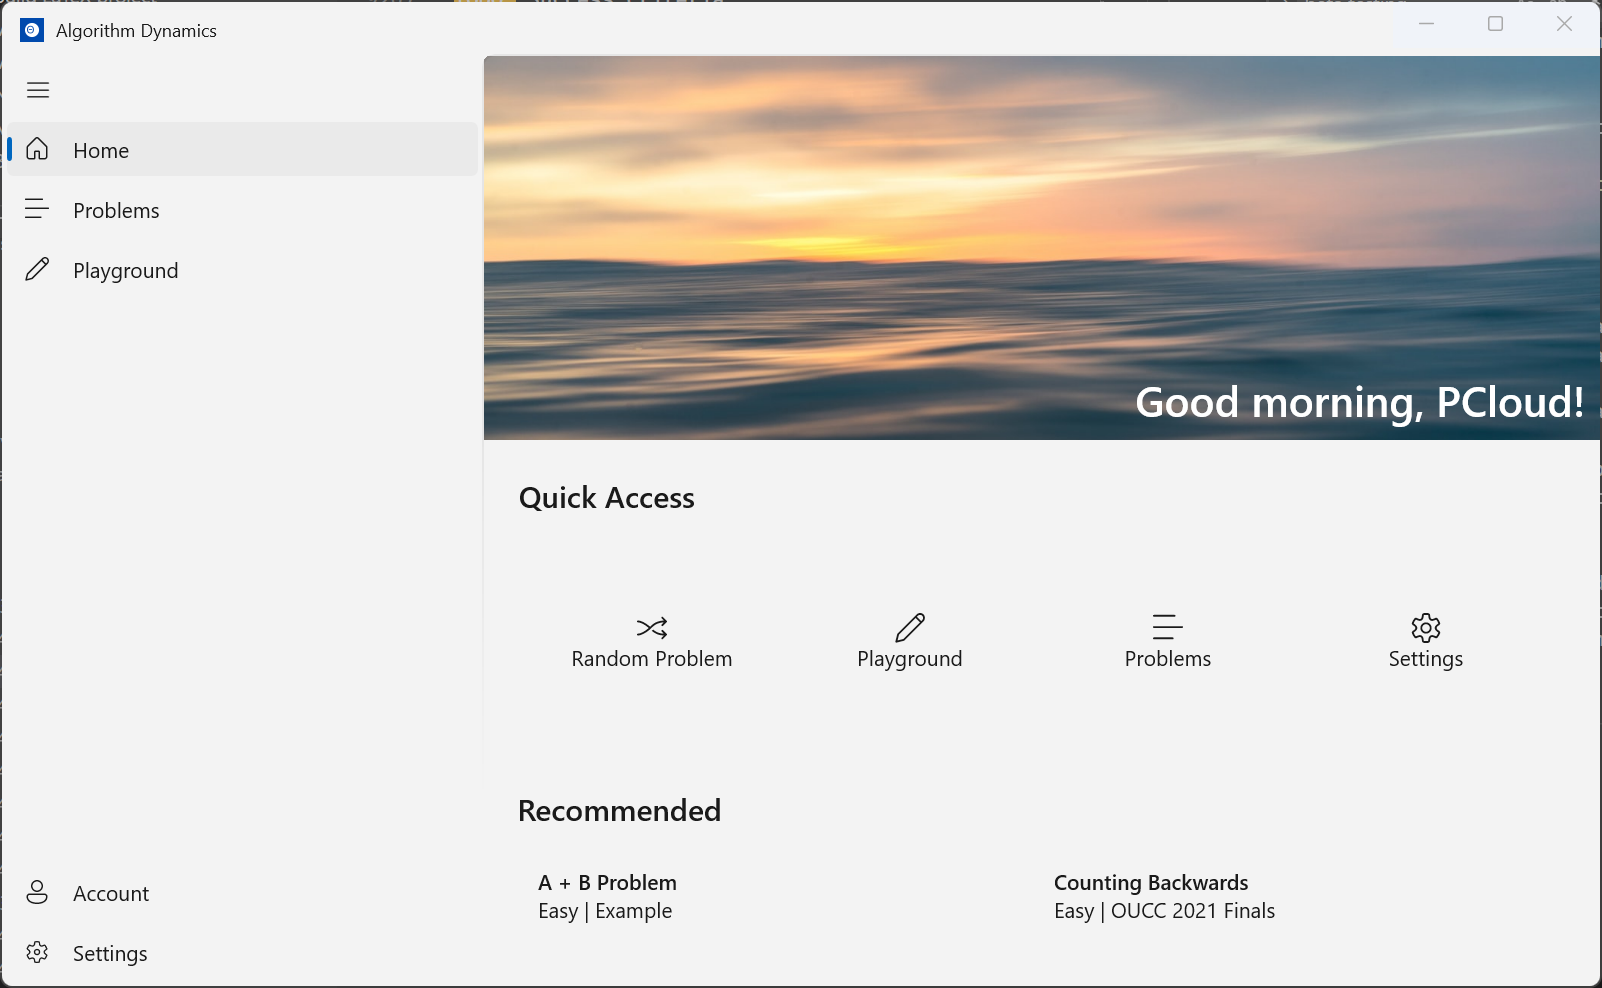
\includegraphics[width=\textwidth, height=\textheight, keepaspectratio]{HomePage-Final}

Now, when I click the random problem button or the recommendations button, I am navigated to the correct problem correctly.

On the ProblemsPage, I first set up the RefreshDatabase method. It loads all data from the database for further queries.

\begin{minted}{csharp}
/// <summary>
/// Reload all data from the database
/// </summary>
private void RefreshDatabase()
{
    // Clear the existing lists
    ProblemLists.Clear();
    Tags.Clear();
    Problems.Clear();

    // Load all data from the database
    Problem.All.ForEach(problem => Problems.Add(problem));
    Core.Models.Tag.All.ForEach(tag => Tags.Add(tag));
    ProblemList.All.ForEach(problemList => ProblemLists.Add(problemList));
}
\end{minted}

I implement the DeleteProblem method, it shows up a dialogue and deletes the selected problem.

\begin{minted}{csharp}
/// <summary>
/// Show a content dialog to confirm the deletion of Problems
/// </summary>
/// <param name="sender"></param>
/// <param name="e"></param>
/// <exception cref="NotImplementedException"></exception>
private async void DeleteProblems(object sender, RoutedEventArgs e)
{
    ContentDialog dialog = new()
    {
        Title = "Delete Problem",
        PrimaryButtonText = "Delete",
        CloseButtonText = "Cancel",
        Content = $"Are you sure that you want to permanently delete these {ProblemsListView.SelectedItems.Count} Problems?",
        DefaultButton = ContentDialogButton.Close,
        XamlRoot = Content.XamlRoot
    };
    var result = await dialog.ShowAsync();
    if (result == ContentDialogResult.Primary)
    {
        var problems = ProblemsListView.SelectedItems;
        foreach (Problem problem in problems) problem.Delete();
        RefreshDatabase();
    }
}
\end{minted}

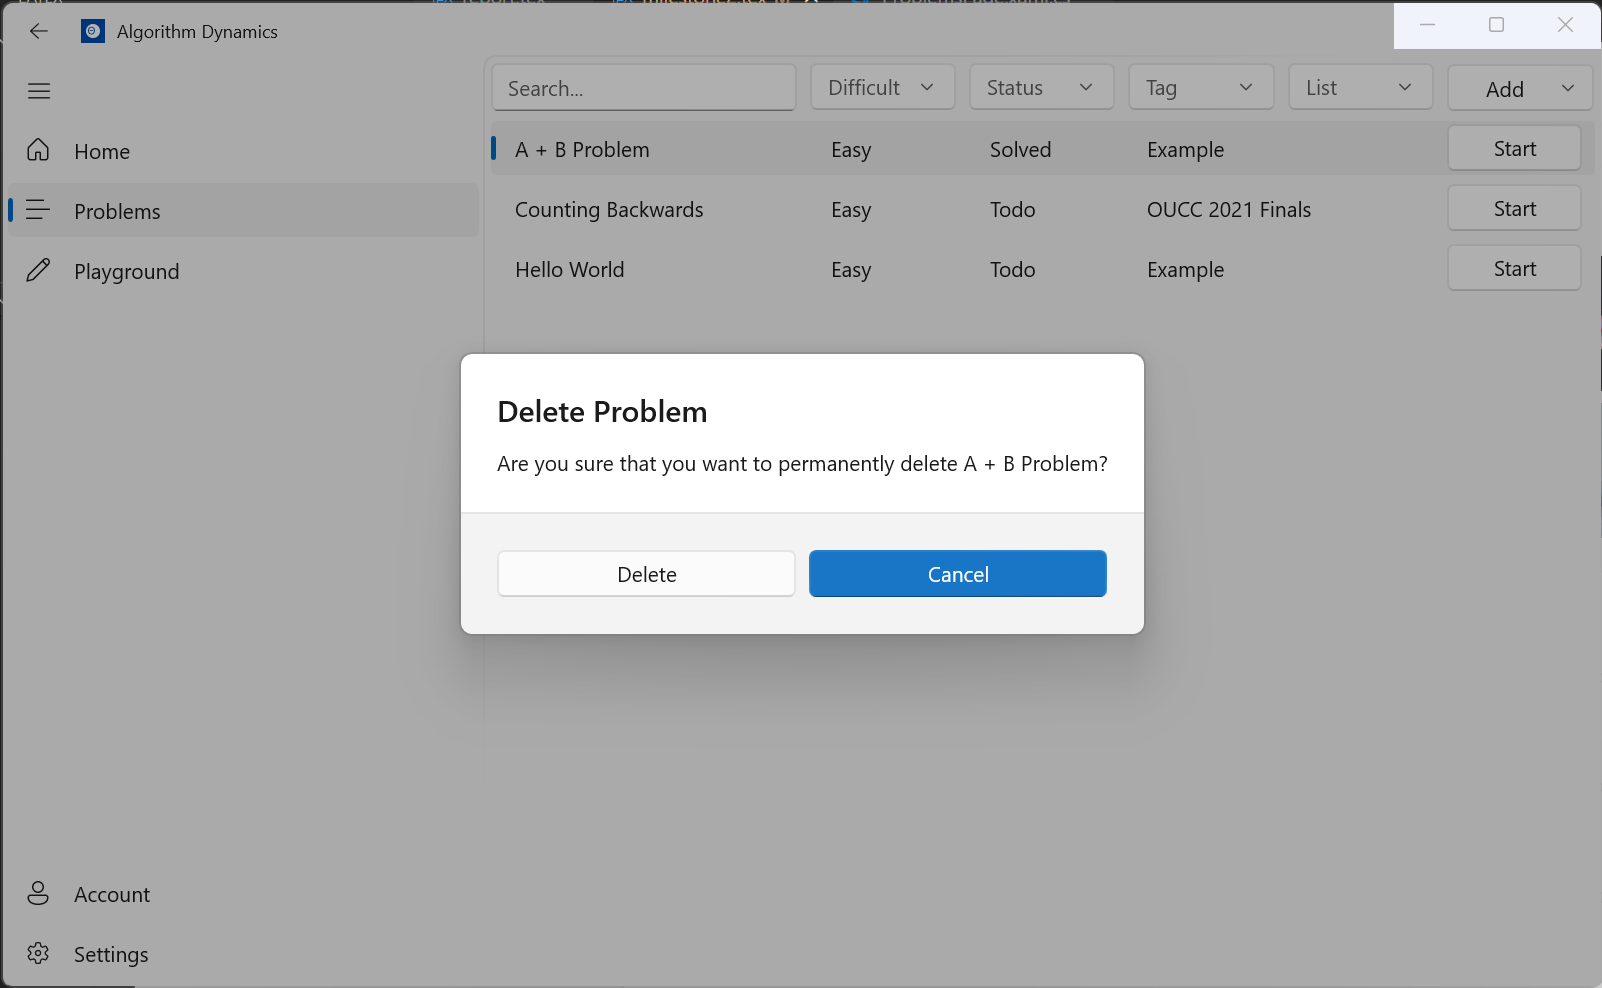
\includegraphics[width=\textwidth, height=\textheight, keepaspectratio]{ProblemsPage-Delete}

Next, I need to implement the search function. When the search box is submitted or the combo box is selected, a Query function is executed and return the search result.

\begin{minted}{csharp}
/// <summary>
/// Trigger when the search box is submitted
/// </summary>
private void Search(AutoSuggestBox sender, AutoSuggestBoxQuerySubmittedEventArgs args)
    => Query();

/// <summary>
/// Trigger when the combo box is changed
/// </summary>
private void Search(object sender, SelectionChangedEventArgs e)
    => Query();

private void Query()
{
    // Clear existing results
    Problems.Clear();
    NoResultTextBlock.Visibility = Visibility.Collapsed;
    
    // Get all problems
    var problems = Problem.All;

    // Query difficulty
    if (DifficultyComboBox.SelectedIndex != -1)
    {
        var difficulty = (Difficulty)DifficultyComboBox.SelectedIndex;
        problems.RemoveAll(p => p.Difficulty != difficulty);
    }

    // Query status
    if (StatusComboBox.SelectedIndex != -1)
    {
        var status = (ProblemStatus)StatusComboBox.SelectedIndex;
        problems.RemoveAll(p => p.Status != status);
    }

    // Query tag
    if (TagComboBox.SelectedIndex != -1)
    {
        var tag = (Tag)TagComboBox.SelectedItem;
        problems.RemoveAll(p => p.Tags.Contains(tag) == false);
    }

    // Query list
    if (ListComboBox.SelectedIndex != -1)
    {
        var list = (ProblemList)ListComboBox.SelectedItem;
        problems.RemoveAll(p => list.Problems.Contains(p) == false);
    }

    // Query name
    if (string.IsNullOrEmpty(ProblemsSearchBox.Text) == false)
    {
        var name = ProblemsSearchBox.Text;
        problems.RemoveAll(p => p.Name != name);
    }

    // Handle no result
    if (problems.Count == 0)
        NoResultTextBlock.Visibility = Visibility.Visible;

    // Return results
    foreach (var problem in problems)
    {
        Problems.Add(problem);
    }
}
\end{minted}

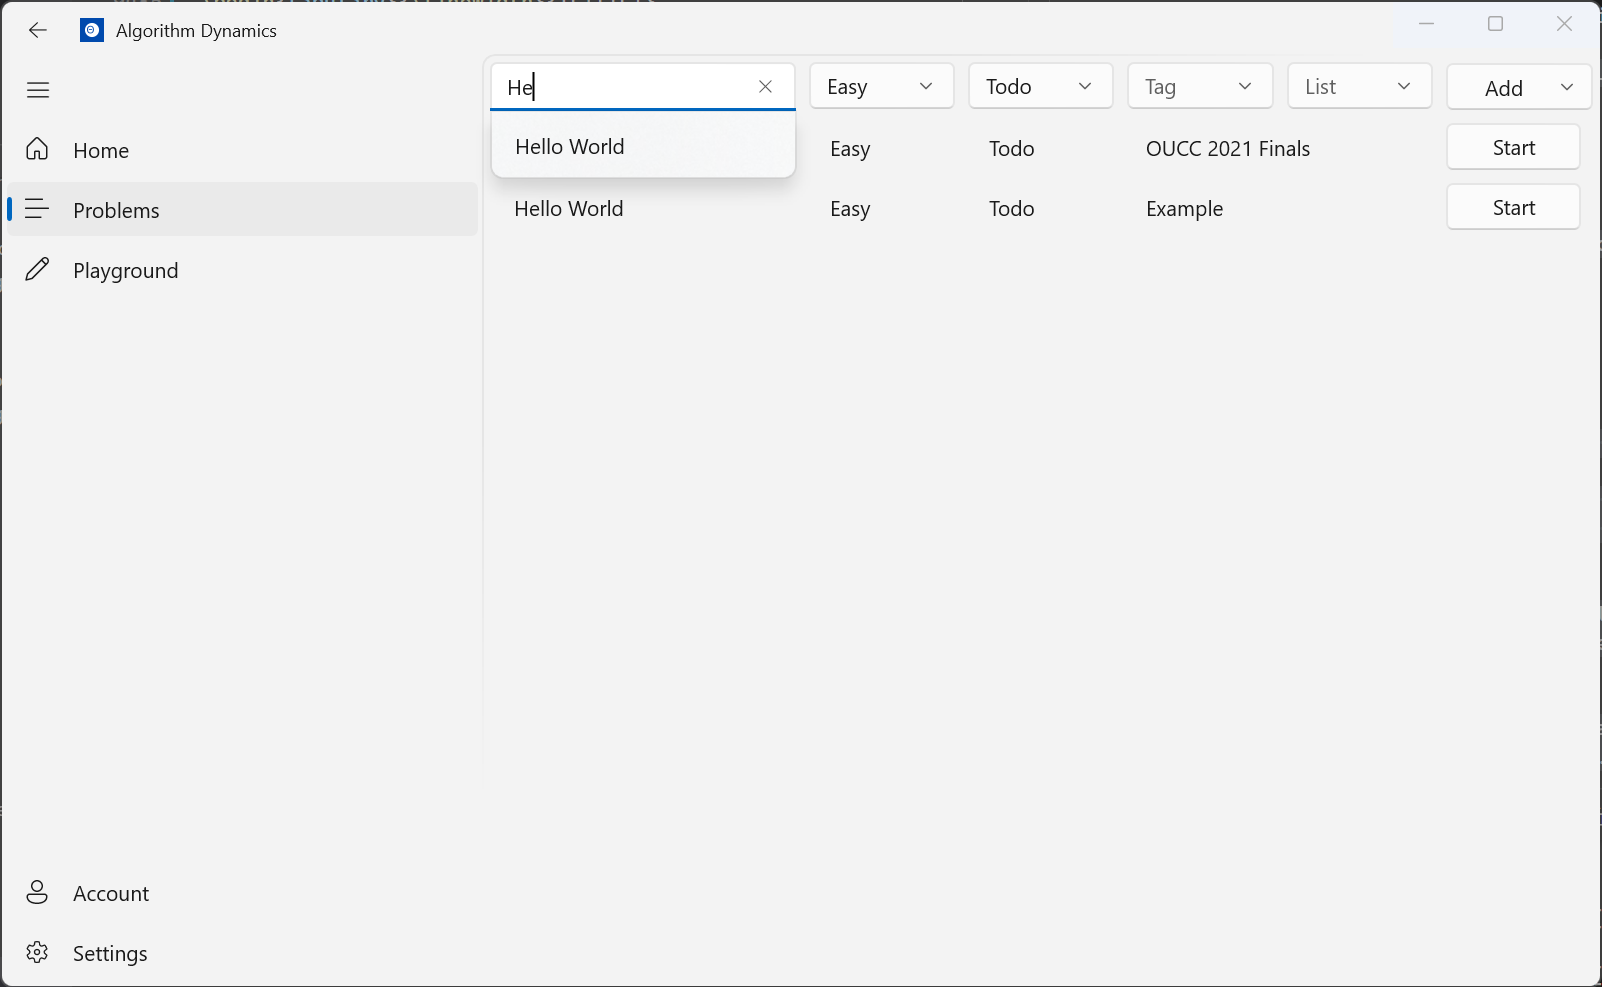
\includegraphics[width=\textwidth, height=\textheight, keepaspectratio]{ProblemsPage-Testing-Search}

When the user is inputting in the search box, the fuzzy search provides suggestions in the drop-down menu. The exact algorithm is explained in the design chapter.

\begin{minted}{csharp}
/// <summary>
/// Give fuzzy search suggestions when the user is inputing search query
/// </summary>
/// <param name="sender"></param>
/// <param name="args"></param>
private void ProblemsSearchBox_TextChanged(AutoSuggestBox sender, AutoSuggestBoxTextChangedEventArgs args)
{
    // Query if empty
    if (string.IsNullOrEmpty(ProblemsSearchBox.Text))
    {
        Query();
    }
    else
    {
        // Give fuzzy search suggestions
        string keyword = ProblemsSearchBox.Text.Trim();
        var resultList = new List<Problem>();
        var sourceList = Problem.All;
        var splitKeyword = keyword.ToLower().Split(' ');
        for (int i = 0; i < sourceList.Count; i++)
        {
            for (int j = 0; j < splitKeyword.Length; j++)
            {
                var sourceKey = sourceList[i].Name.ToLower();
                if (sourceKey.Contains(splitKeyword[j]))
                {
                    resultList.Add(sourceList[i]);
                    break;
                }
            }
        }
        // Return result
        sender.ItemsSource = resultList.Select(p => p.Name).ToList();
    }
}
\end{minted}

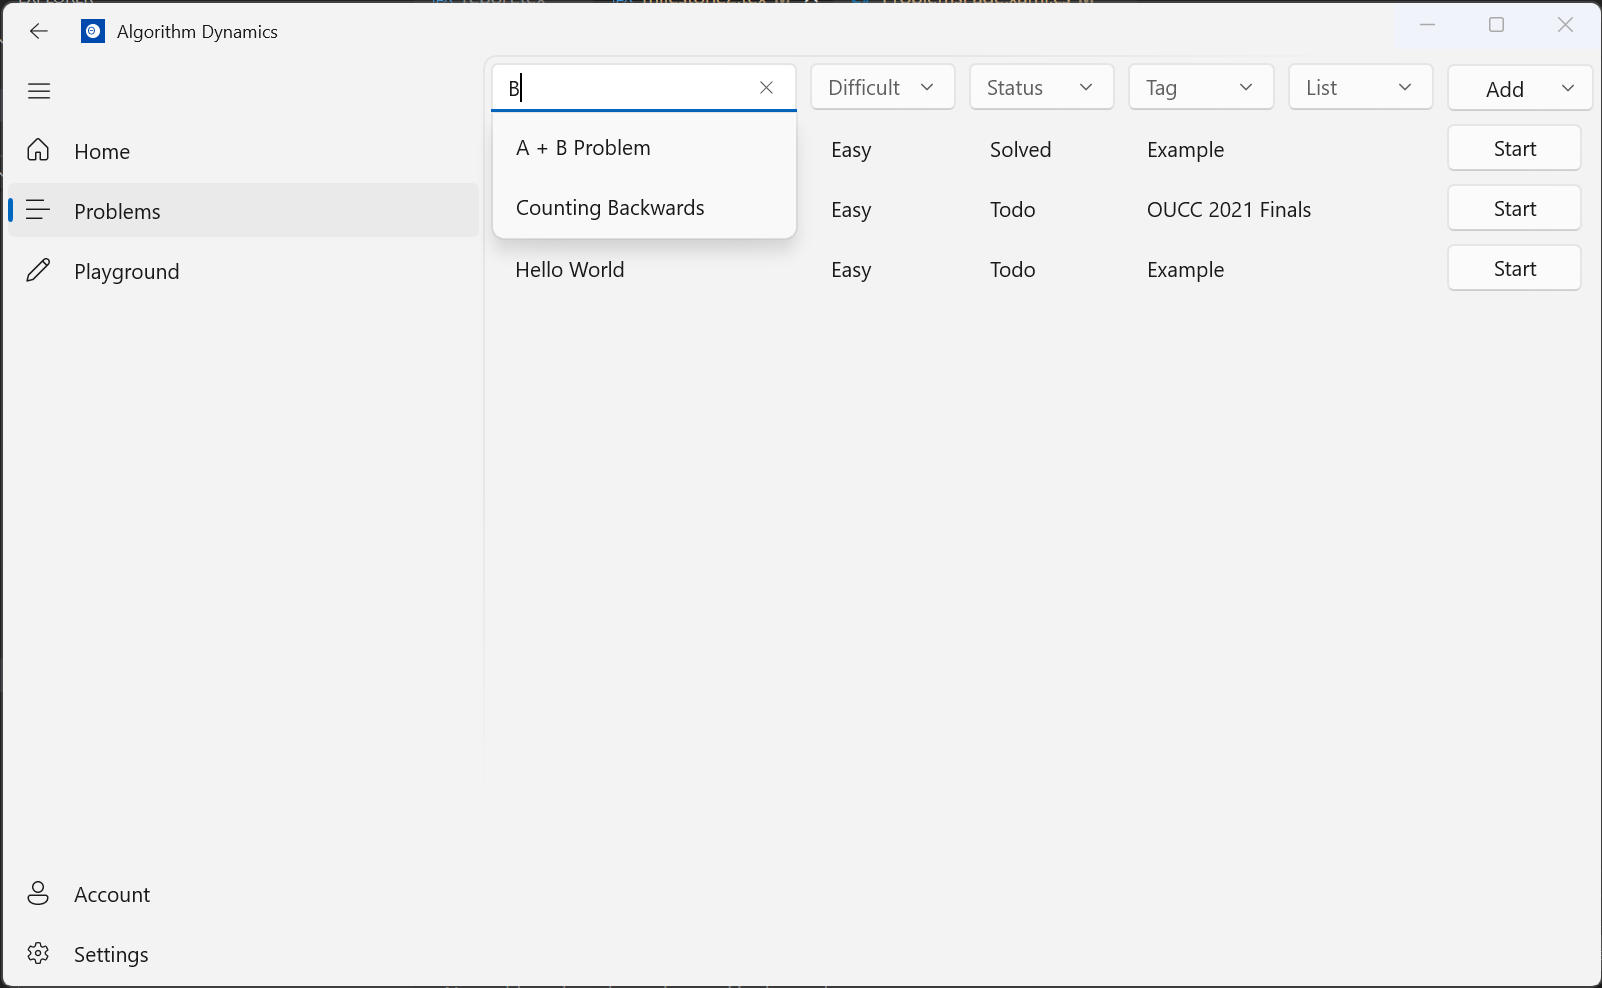
\includegraphics[width=\textwidth, height=\textheight, keepaspectratio]{ProblemsPage-FuzzySearch}

Next, I integrate the CreateNew pages. I will show the CreateNewProblemListPage as an example since both of them share a similar process, please refer to the source code for details.

The key to the integration is to create a new problem list and save any changes to the database.

\begin{minted}{csharp}
/// <summary>
/// When the save button is clicked, save the problem list and change the description test.
/// </summary>
/// <param name="sender"></param>
/// <param name="e"></param>
private void SaveButton_Click(object sender, RoutedEventArgs e)
{
    if (_pageMode == Mode.CreateProblemList)
    {
        _problemList = ProblemList.Create(_name, _description, Problems.ToList());
    }
    else if (_pageMode == Mode.EditProblemList)
    {
        // Save name
        _problemList.Name = _name;
        // Save description
        _problemList.Description = _description;
        // Save problems
        Problems.ToList().ForEach(problem =>
        {
            if (_problemList.Problems.Contains(problem) == false)
            {
                _problemList.AddProblem(problem);
            }
        });
        _problemList.Problems.ToList().ForEach(problem =>
        {
            if (Problems.Contains(problem) == false)
            {
                _problemList.RemoveProblem(problem);
            }
        });
    }

    // Done
    TestTextBlock.Text = "The Problem List is saved.";
}
\end{minted}

I also need to add validation to all the fields to ensure none of them is empty.

\begin{minted}{csharp}
public bool IsValidInput
{
    get
    {
        ErrorMessage = "";
        bool isValid = true;
        if (string.IsNullOrEmpty(_name))
        {
            isValid = false;
            ErrorMessage += "A name is required.\n";
        }
        if (Problems.Count < 1)
        {
            isValid = false;
            ErrorMessage += "At least one problem is required.\n";
        }
        return isValid;
    }
}
\end{minted}

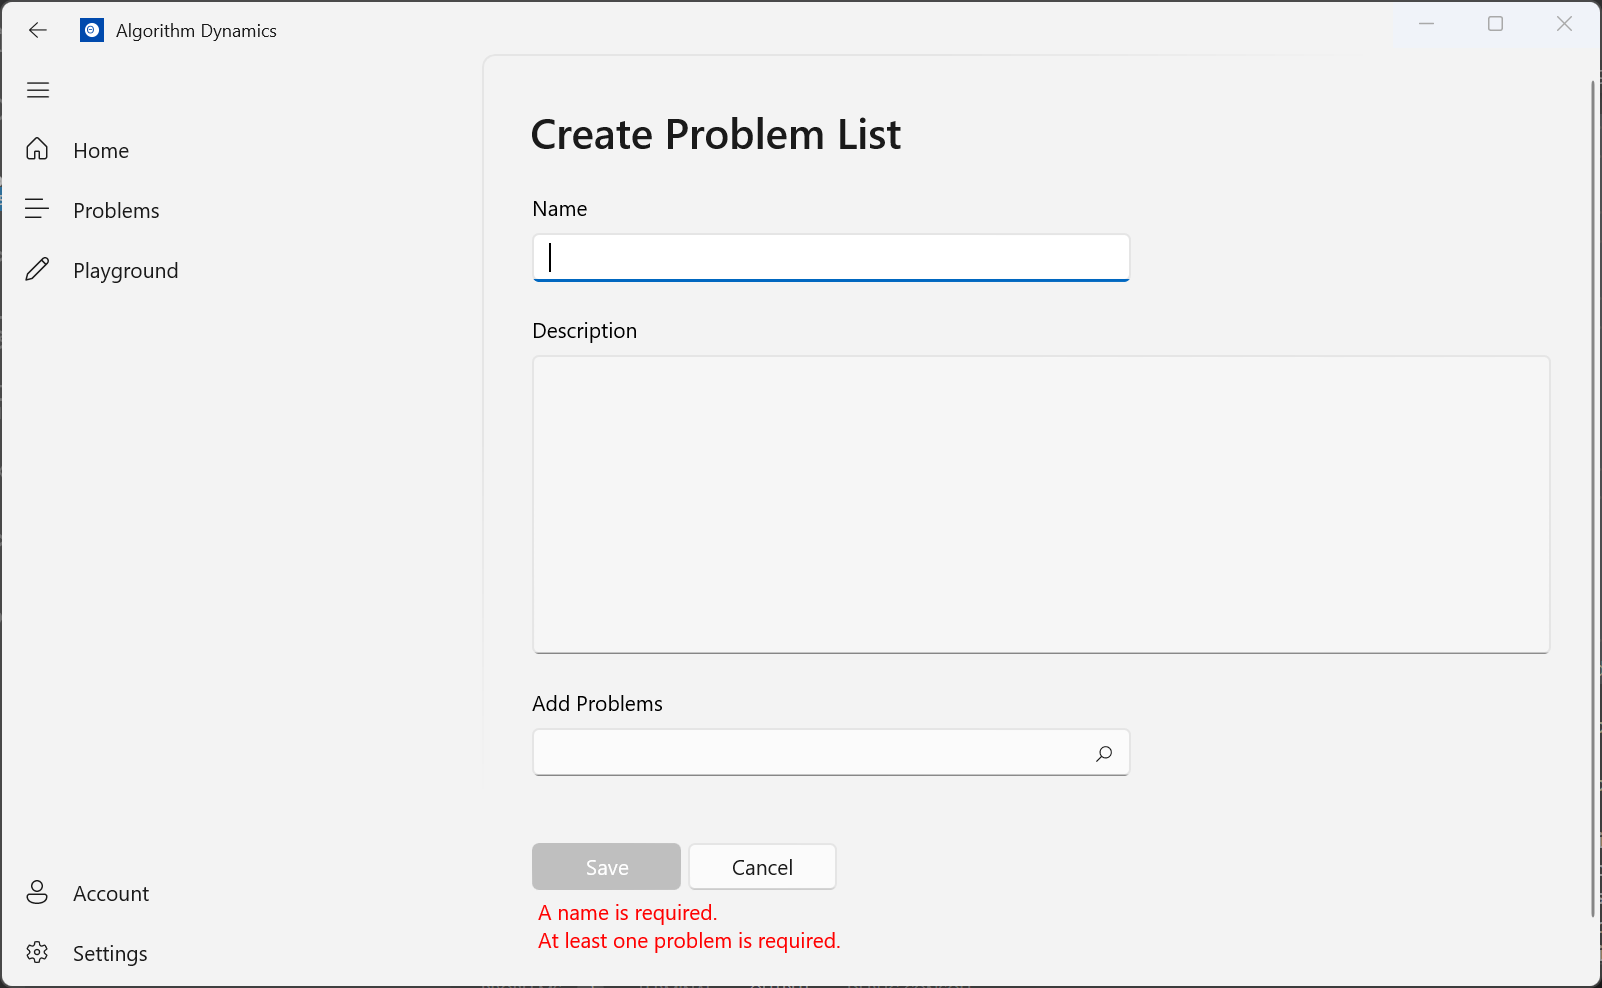
\includegraphics[width=\textwidth, height=\textheight, keepaspectratio]{CreateNewProblemListPage-Testing-Empty}

In the CodingPage Integration, I need to render the given problem into a markdown file, so it can be displayed with all formats supported.

\begin{minted}{csharp}
/// <summary>
/// The renderec markdown text of the current problem
/// </summary>
public string ProblemMarkdown
{
    get
    {
        if (_currentProblem != null)
        {
            const int MB = 1024 * 1024;
            
            // Set title
            string title = $"# {_currentProblem.Name}\n";
            
            // Set time limit
            string timeLimit = $"\n## Time Limit\n{_currentProblem.TimeLimit} ms";
            
            // Set memory limit
            string memoryLimit = $"\n## Memory Limit\n{_currentProblem.MemoryLimit / MB} MB";
            
            // Set example test case
            string example = "\n## Example";
            int testCaseCnt = 1;
            _currentProblem.TestCases.Where(testCase => testCase.IsExample == true).ToList().ForEach(testCase =>
            {
                example += $"\n### Example Input {testCaseCnt}\n";
                example += "```\n" + testCase.Input.Replace("\n", "\n") + "\n```\n";
                example += $"\n### Example Output {testCaseCnt}\n";
                example += "```\n" + testCase.Output.Replace("\n", "\n") + "\n```\n";
                testCaseCnt++;
            });

            return title + _currentProblem.Description + timeLimit + memoryLimit + example;
        }
        return "";
    }
}
\end{minted}

I use the test data in the design section to test the markdown renderer. However, the data is not rendered as expected. There is no line break, and all text is rendered as the title.

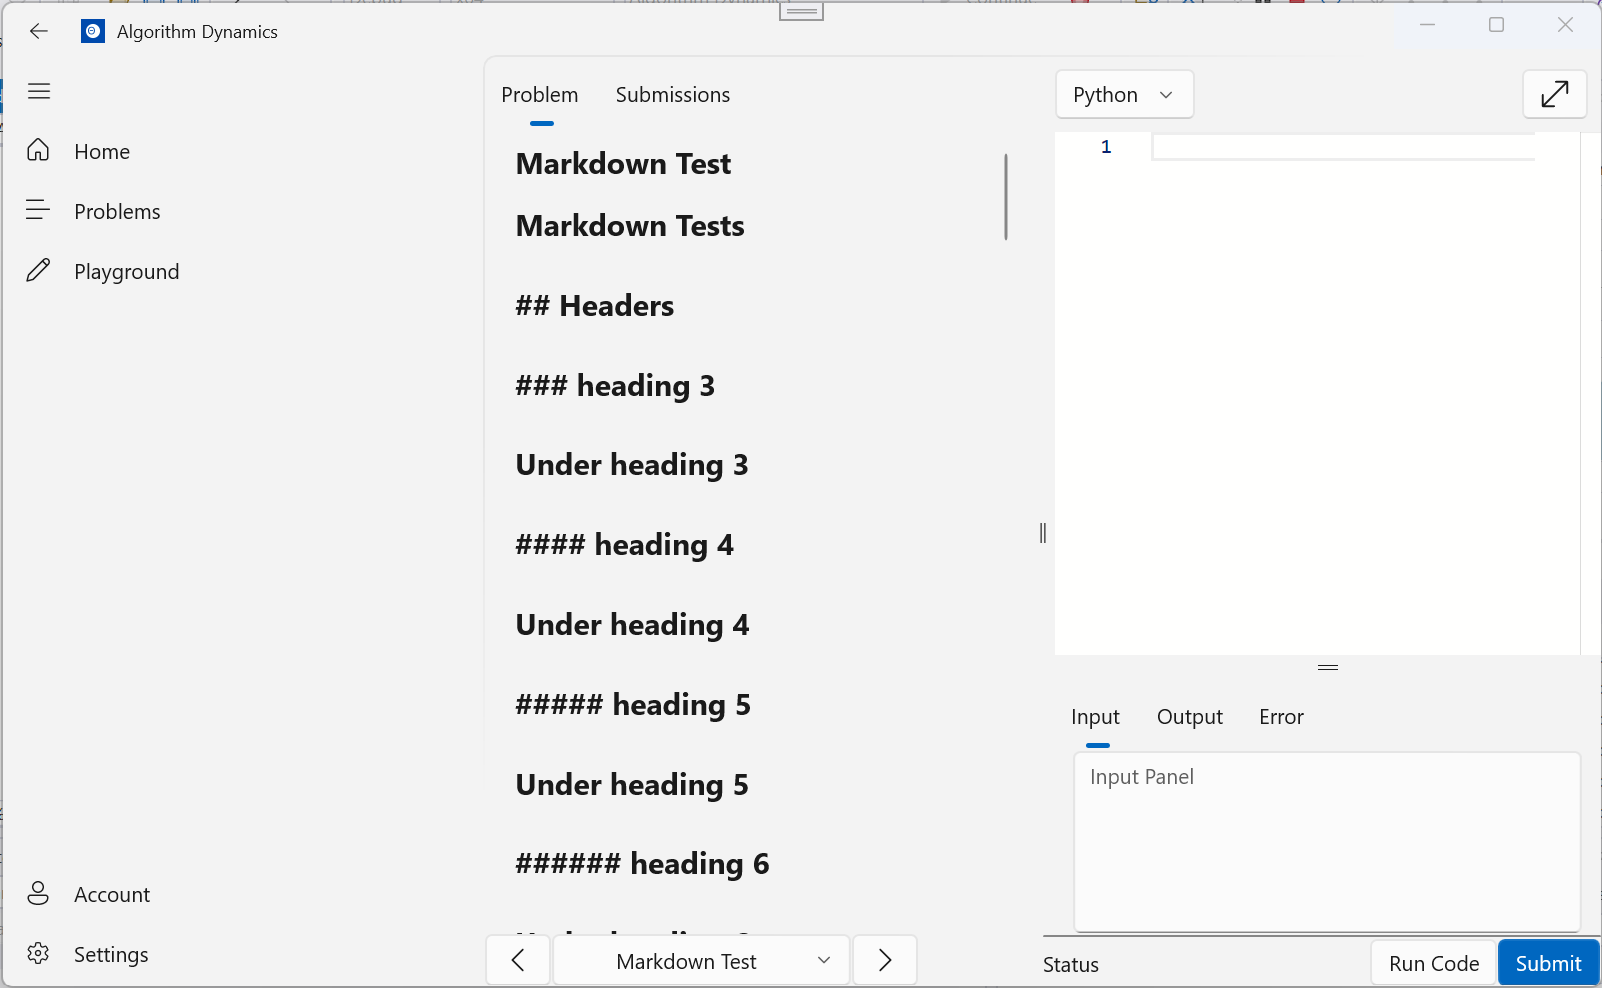
\includegraphics[width=\textwidth, height=\textheight, keepaspectratio]{CodingPage-MarkdownTest-Failed}

After some debugging and reading the documentation of the markdown control, I found that I should use `\\r' instead of `\\n' for newlines.

\begin{minted}{csharp}
/// <summary>
/// The renderec markdown text of the current problem
/// </summary>
public string ProblemMarkdown
{
    get
    {
        if (_currentProblem != null)
        {
            const int MB = 1024 * 1024;
            
            // Set title
            string title = $"# {_currentProblem.Name}\r";
            
            // Set time limit
            string timeLimit = $"\r## Time Limit\r{_currentProblem.TimeLimit} ms";
            
            // Set memory limit
            string memoryLimit = $"\r## Memory Limit\r{_currentProblem.MemoryLimit / MB} MB";
            
            // Set example test case
            string example = "\r## Example";
            int testCaseCnt = 1;
            _currentProblem.TestCases.Where(testCase => testCase.IsExample == true).ToList().ForEach(testCase =>
            {
                example += $"\r### Example Input {testCaseCnt}\r";
                example += "```\r" + testCase.Input.Replace("\r", "\r") + "\r```\r";
                example += $"\r### Example Output {testCaseCnt}\r";
                example += "```\r" + testCase.Output.Replace("\r", "\r") + "\r```\r";
                testCaseCnt++;
            });

            return title + _currentProblem.Description + timeLimit + memoryLimit + example;
        }
        return "";
    }
}
\end{minted}

The markdown renderer works correctly now.

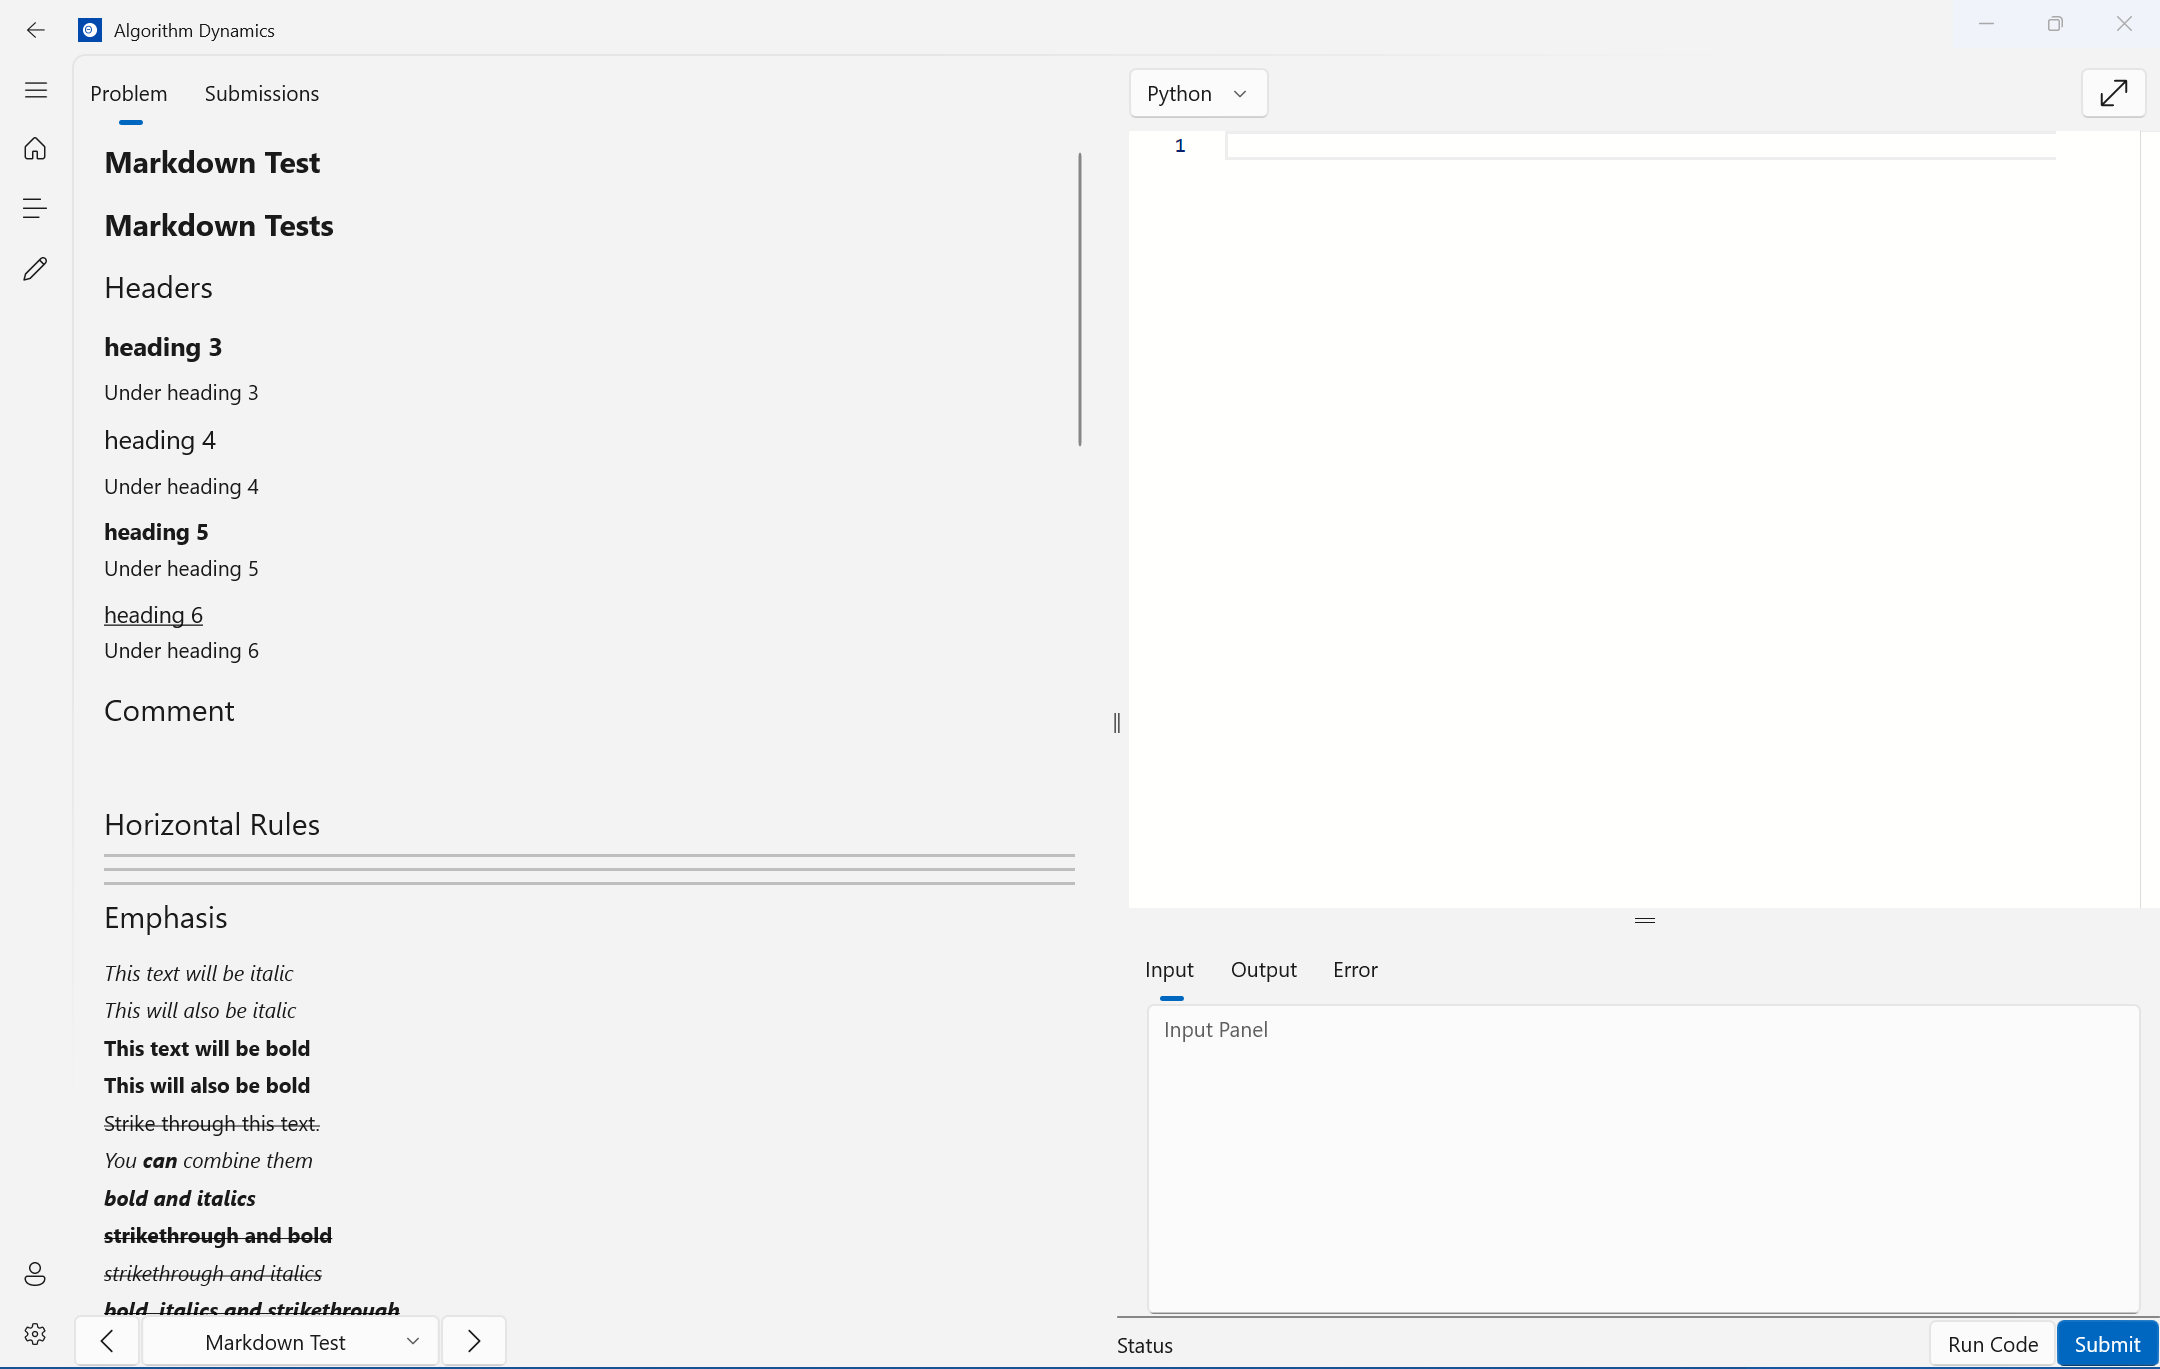
\includegraphics[width=\textwidth, height=\textheight, keepaspectratio]{CodingPage-MarkdownTest}

For the submission grid, I can directly bind it to the list of submissions and it will get updated automatically when a new submission is created.

\begin{minted}{xml}
<controls:DataGrid
    x:Name="SubmissionsDataGrid"
    AutoGenerateColumns="False"
    IsReadOnly="True"
    SelectionMode="Single"
    CanUserReorderColumns="False"
    MinColumnWidth="100"
    SelectionChanged="SubmissionsDataGrid_SelectionChanged"
    ItemsSource="{x:Bind ReverseSubmissions, Mode=OneWay}">
    <controls:DataGrid.Columns>
    <controls:DataGridTextColumn
        Header="Submit Time"
        Width="SizeToCells"
        Binding="{Binding Submission.SubmittedTime}"/>
    <controls:DataGridComboBoxColumn
        Header="Status"
        Width="SizeToCells"
        Binding="{Binding Result}"/>
    <controls:DataGridComboBoxColumn
        Header="Runtime"
        Width="SizeToCells"
        Binding="{Binding CPUTimeAsString}"/>
    <controls:DataGridComboBoxColumn
        Header="Memory"
        Width="SizeToCells"
        Binding="{Binding MemoryUsageAsString}"/>
    <controls:DataGridComboBoxColumn
        Header="Language"
        Width="SizeToCells"
        Binding="{Binding Submission.Language.DisplayName}"/>
    </controls:DataGrid.Columns>
</controls:DataGrid>
\end{minted}

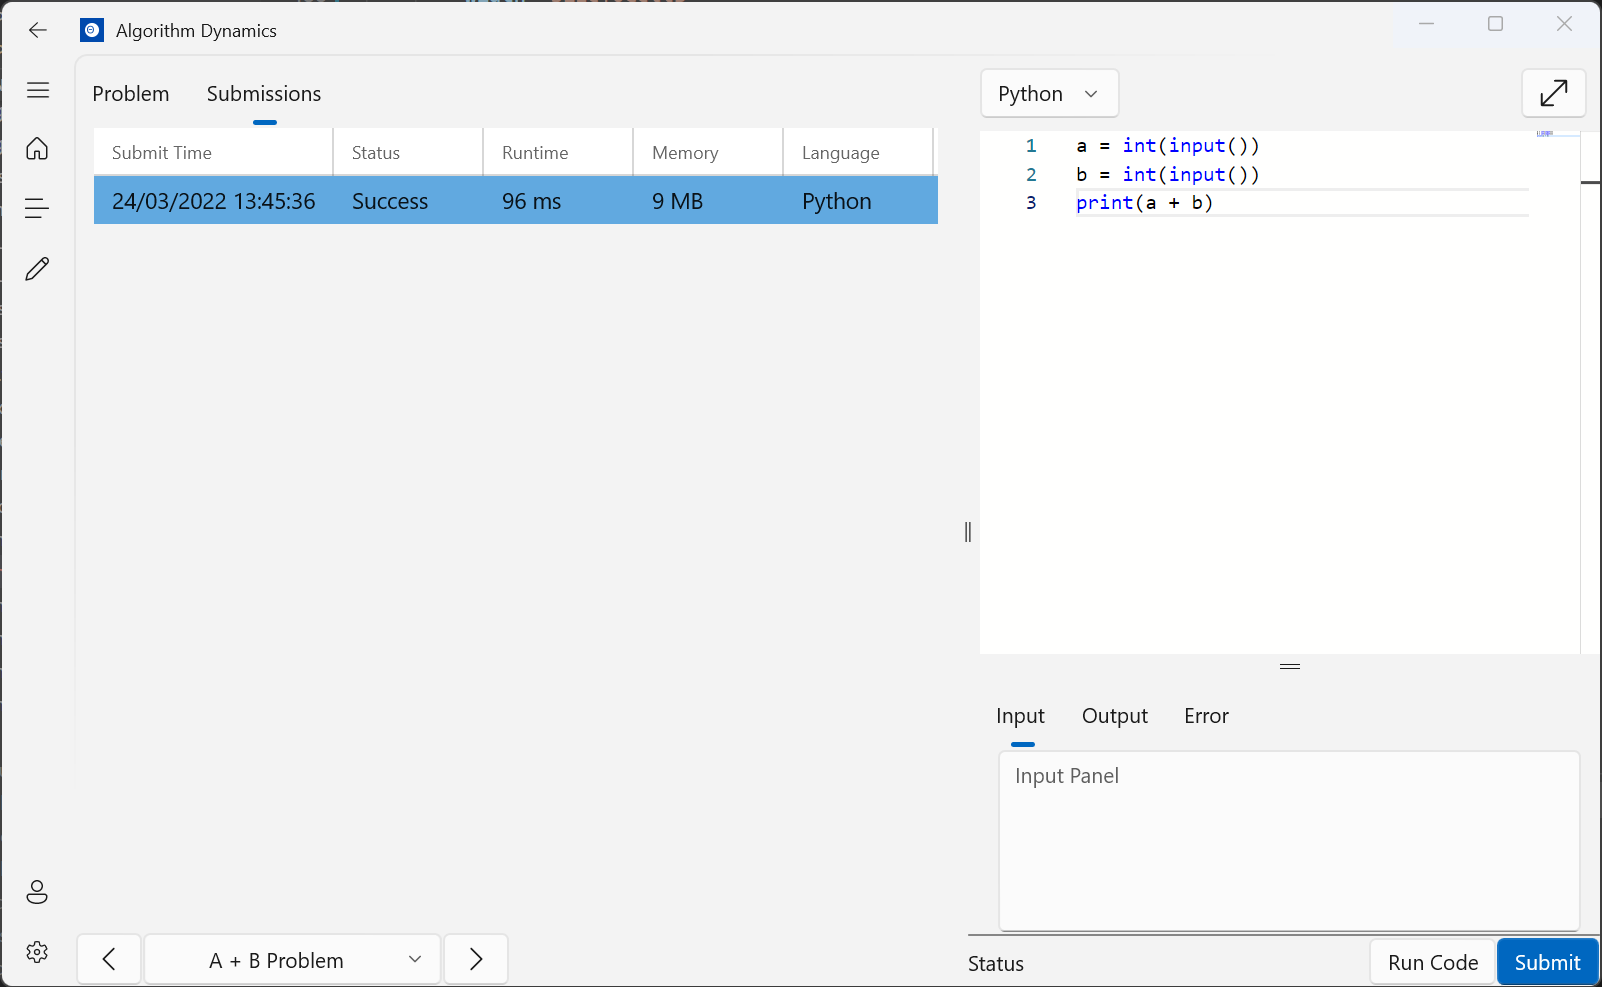
\includegraphics[width=\textwidth, height=\textheight, keepaspectratio]{CodingPage-SubmissionGrid}

Finally, I need to integrate the AccountPage. The main job is to generate all statistics for the current user. The InitializeStatsItems procedure is called when the constructor of the Page is executed, so the statistics are generated when the page is loaded. It reads from the database and performs the calculations and save the results.

\begin{minted}{csharp}
public AccountPage()
{
    InitializeComponent();
    InitializeStatsItems();
}
/// <summary>
/// Initialize the statistics items
/// </summary>
private void InitializeStatsItems()
{
    // Count all problems solved
    StatsItems.Add(new("Problem Solved", Problem.All.Count(problem => problem.Status == ProblemStatus.Solved).ToString()));
    
    // Count all problems attempted
    StatsItems.Add(new("Problem Attempted", Problem.All.Count(problem => problem.Status == ProblemStatus.Attempted).ToString()));
    
    // Count all problems todo
    StatsItems.Add(new("Problem Todo", Problem.All.Count(problem => problem.Status == ProblemStatus.Todo).ToString()));

    // Count correct rate
    StatsItems.Add(new("Correct Rate", $"{(SubmissionResult.All.Count(result => result.ResultCode == ResultCode.SUCCESS) * 100 / Submission.All.Count)}%"));

    // Count the favourite tag
    string favTag = "";
    int maxTag = 0;
    foreach (var tag in Core.Models.Tag.All)
    {
        int tagCnt = Submission.All.Count(submission => submission.Problem.Tags.Contains(tag));
        if (tagCnt > maxTag)
        {
            maxTag = tagCnt;
            favTag = tag.Name;
        }
    }
    StatsItems.Add(new("Favourite Topic", favTag));

    // Count the favourite language
    string favLang = "";
    int maxLang = 0;
    foreach (var lang in Core.Models.Language.All)
    {
        int langCnt = Submission.All.Count(submission => Equals(submission.Language, lang));
        if (langCnt > maxLang)
        {
            maxLang = langCnt;
            favLang = lang.DisplayName;
        }
    }
    StatsItems.Add(new("Favourite Language", favLang));
}
\end{minted}

When I first run the app, it crashes when I navigated to the AccountPage. The following error message is thrown.

\begin{minted}{text}
System.DivideByZeroException
  HResult=0x80020012
  Message=Attempted to divide by zero.
  Source=Algorithm Dynamics
  StackTrace:
   at Algorithm_Dynamics.Pages.AccountPage.InitializeStatsItems() in C:\Algorithm-Dynamics\src\Algorithm Dynamics\Pages\AccountPage.xaml.cs:line 134
   at Algorithm_Dynamics.Pages.AccountPage..ctor() in C:\Algorithm-Dynamics\src\Algorithm Dynamics\Pages\AccountPage.xaml.cs:line 20
   at Algorithm_Dynamics.Algorithm_Dynamics_XamlTypeInfo.XamlTypeInfoProvider.Activate_59_AccountPage() in C:\Algorithm-Dynamics\src\Algorithm Dynamics\obj\x64\Debug\net6.0-windows10.0.19041.0\XamlTypeInfo.g.cs:line 567
   at Algorithm_Dynamics.Algorithm_Dynamics_XamlTypeInfo.XamlUserType.ActivateInstance() in C:\Algorithm-Dynamics\src\Algorithm Dynamics\obj\x64\Debug\net6.0-windows10.0.19041.0\XamlTypeInfo.g.cs:line 7704
   at ABI.Microsoft.UI.Xaml.Markup.IXamlType.Do_Abi_ActivateInstance_13(IntPtr thisPtr, IntPtr* result)

  This exception was originally thrown at this call stack:
    Algorithm_Dynamics.Pages.AccountPage.InitializeStatsItems() in AccountPage.xaml.cs
    Algorithm_Dynamics.Pages.AccountPage.AccountPage() in AccountPage.xaml.cs
    Algorithm_Dynamics.Algorithm_Dynamics_XamlTypeInfo.XamlTypeInfoProvider.Activate_59_AccountPage() in XamlTypeInfo.g.cs
    Algorithm_Dynamics.Algorithm_Dynamics_XamlTypeInfo.XamlUserType.ActivateInstance() in XamlTypeInfo.g.cs
    ABI.Microsoft.UI.Xaml.Markup.IXamlType.Do_Abi_ActivateInstance_13(System.IntPtr, System.IntPtr*)
\end{minted}

It is a divide by zero error because the number of submissions is 0. I can fix this by adding branching to handle the 0 cases.

\begin{minted}{csharp}
// Count correct rate
if (Submission.All.Count > 0)
{
    StatsItems.Add(new("Correct Rate", $"{(SubmissionResult.All.Count(result => result.ResultCode == ResultCode.SUCCESS) * 100 / Submission.All.Count)}%"));
}
else
{
    StatsItems.Add(new("Correct Rate", "0%"));
}
\end{minted}

Now the AccountPage works correctly with all statistics showing up correctly.

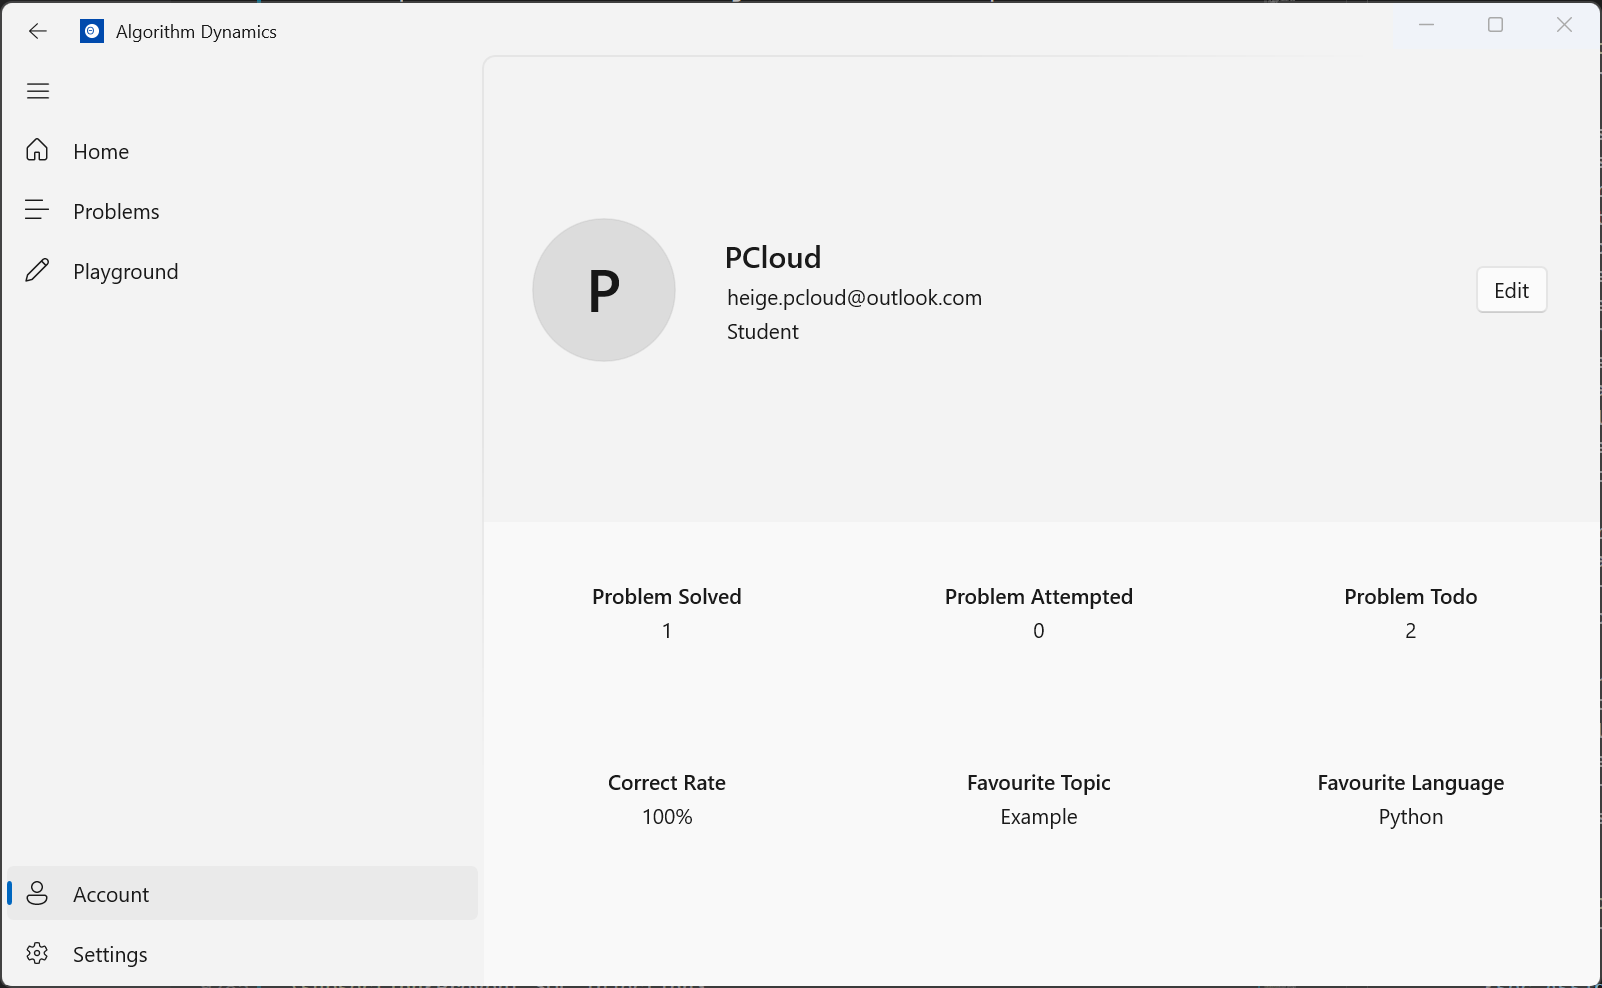
\includegraphics[width=\textwidth, height=\textheight, keepaspectratio]{AccountPage-Final.png}}

\subsubsection{Stakeholder feedback}

Mr Grimwood asked me what will happen to the account page when the software is installed for the first time. Where does the user create an account? In my current design, there is no such sign-up page. I think when the app launches if it finds there is no user in the database, it should promote the user to a registration page. The user can only log in after registration.

I place the welcome page in the main window.

\begin{minted}{xml}
<!--WelcomePage for creating new user on first startup-->
<Grid
    Grid.Row="1"
    x:Name="WelcomeGrid"
    Visibility="Collapsed"
    Background="{ThemeResource ApplicationPageBackgroundThemeBrush}">
    <StackPanel
    VerticalAlignment="Center"
    HorizontalAlignment="Center">
    <TextBlock 
        Margin="32"
        Style="{ThemeResource TitleTextBlockStyle}"
        Text="Welcome to Algorithm Dynamics"/>
    <TextBox
        Header="Your Name"
        Margin="8"
        MaxWidth="200"
        PlaceholderText="Name"
        IsSpellCheckEnabled="False"
        Text="{x:Bind UserName, Mode=TwoWay}"/>
    <TextBox
        Header="Your Email"
        Margin="8"
        MaxWidth="200"
        PlaceholderText="Email"
        IsSpellCheckEnabled="False"
        Text="{x:Bind Email, Mode=TwoWay}"/>
    <ComboBox
        Header="Role"
        Margin="8"
        MaxWidth="200"
        HorizontalAlignment="Stretch"
        SelectedIndex="{x:Bind RoleIndex, Mode=TwoWay}">
        <x:String>Student</x:String>
        <x:String>Teacher</x:String>
    </ComboBox>
    <Button 
        x:Name="CreateUserButton"
        Margin="16"
        Content="Go"
        MaxWidth="200"
        HorizontalAlignment="Stretch"
        IsEnabled="{x:Bind IsValidInput, Mode=OneWay}"
        Click="CreateUserButton_Click"/>
    <TextBlock
        Margin="4"
        Text="{x:Bind ErrorMessage, Mode=OneWay}"
        RelativePanel.Below="InputPanel"
        MaxWidth="200"
        RelativePanel.AlignLeftWith="InputPanel"
        Foreground="Red"/>
    </StackPanel>
</Grid>
\end{minted}

In the constructor of the main window, the welcome grid is shown if there is no user in the database.

\begin{minted}{csharp}
public MainWindow()
{
    // ...
    // If no user, show welcome grid
    if (DataAccess.GetAllUsers().Count == 0)
    {
        WelcomeGrid.Visibility = Visibility.Visible;
        UserName = "";
        Email = "";
        Role = 0;
    }
    else
    {
        MainNavView.SelectedItem = MainNavView.MenuItems[0];
    }
}
\end{minted}

When the user clicks the create button, the user is created in the database and the user is navigated to the HomePage.

\begin{minted}{csharp}
/// <summary>
/// Create a new user and store <see cref="User.Uid"/> into settings
/// </summary>
/// <param name="sender"></param>
/// <param name="e"></param>
private void CreateUserButton_Click(object sender, RoutedEventArgs e)
{
    // Create user
    User user = User.Create(UserName, Email, Role);

    // Set current user
    ApplicationDataContainer localSettings = ApplicationData.Current.LocalSettings;
    localSettings.Values["CurrentUser"] = user.Uid;

    // Navigate to HomePage
    WelcomeGrid.Visibility = Visibility.Collapsed;
    MainNavView.SelectedItem = MainNavView.MenuItems[0];
}
\end{minted}

I also set a validation function IsValid. If the user input is not valid, the create button is disabled and a user-friendly error message is displayed.

\begin{minted}{csharp}
/// <summary>
/// Validate the name and the email
/// </summary>
public bool IsValidInput
{
    get
    {
        ErrorMessage = "";
        if (string.IsNullOrEmpty(UserName) || string.IsNullOrEmpty(Email)) 
            return false;
        bool isValid = true;
        if (string.IsNullOrEmpty(UserName))
        {
            isValid = false;
            ErrorMessage += "A user name is required.\n";
        }
        if (IsValidEmail(Email) == false)
        {
            isValid = false;
            ErrorMessage += "The email address is not valid.\n";
        }
        return isValid;
    }
}
\end{minted}

Now, when the user runs the app for the first time, he will be promoted to this registration page.

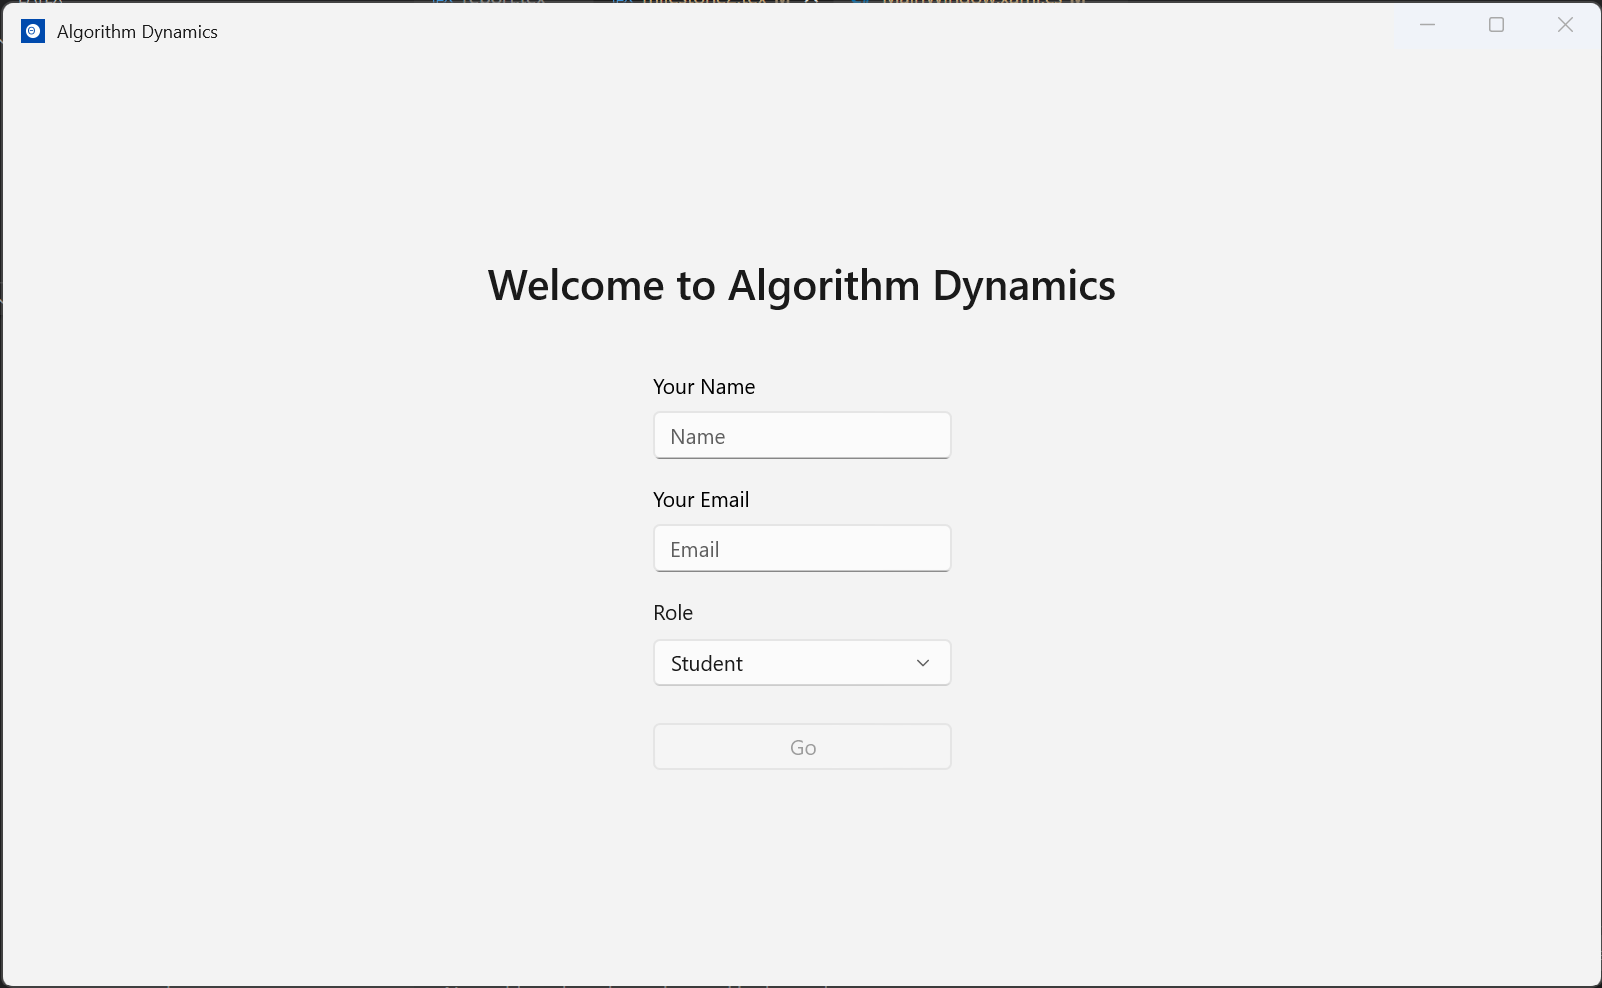
\includegraphics[width=\textwidth, height=\textheight, keepaspectratio]{WelcomeScreen}

Both name and email are validated before the user can continue.

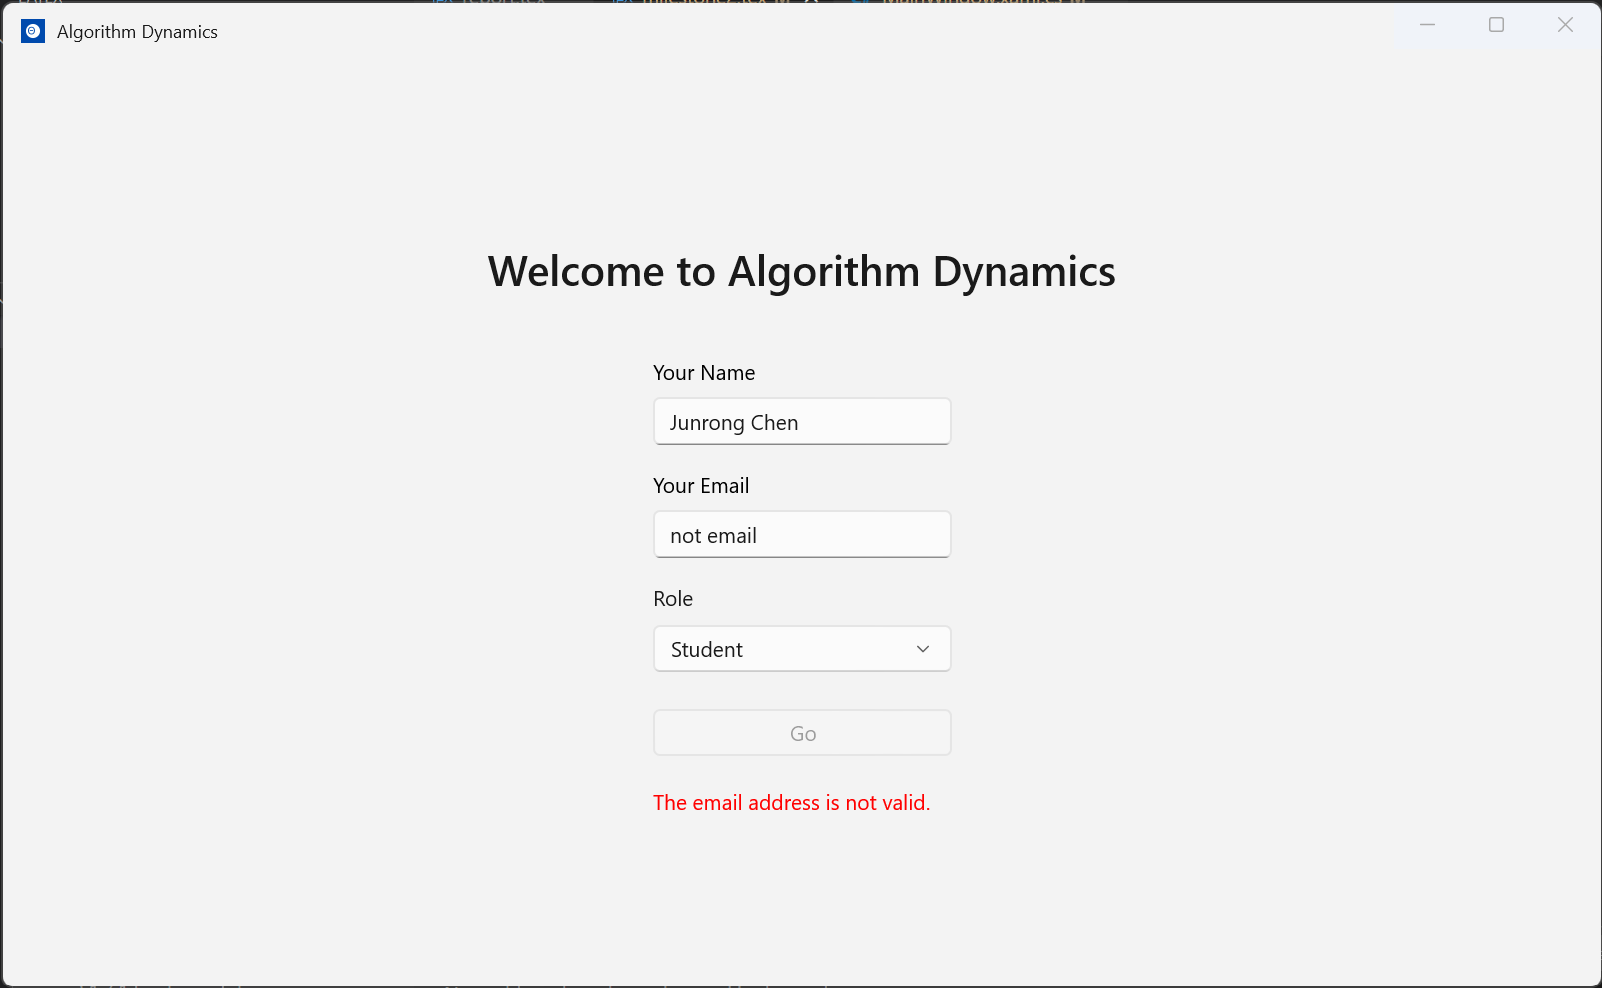
\includegraphics[width=\textwidth, height=\textheight, keepaspectratio]{WelcomeScreen-Validation}

Mr Grimwood is satisfied with the design and the solution.

\end{document}